\documentclass[a4paper]{article}

\usepackage[portuguese,english]{babel}
\usepackage[utf8]{inputenc}
\usepackage[T1]{fontenc}

\newcommand{\documentTitle}{Data Analysis and Transformation \\ TP1: Fundamentals of Signals and Systems}
\newcommand{\pdfTitle}{[ATD] TP1: Fundamentals of Signals and Systems}
\newcommand{\documentAuthors}{José Ribeiro (2008112181, jbaia@student.dei.uc.pt) \\ Pedro Magalhães (2009117002, pjrosa@student.dei.uc.pt)}

\title{\documentTitle}
\author{\documentAuthors}

\usepackage{hyperref}
\hypersetup{
	pdftitle = \pdfTitle
	,pdfauthor = \documentAuthors
	,pdfsubject = {Data Analysis and Transformation}
	,pdfkeywords = {Data Analysis and Transformation} {Signal Processing}
	,pdfborder = {0 0 0}
}

%\usepackage{subfig}
%\usepackage{amsmath}
%\usepackage{array}
\usepackage{anysize}
\usepackage{lscape}
\usepackage{amsmath}
\usepackage{graphicx}
\usepackage{caption}
%\usepackage[pdftex]{graphicx}
%\usepackage[table]{xcolor}

\hyphenation{}

\marginsize{3.5cm}{3.5cm}{3cm}{3cm}

\makeatletter

\begin{document}
\maketitle
\cleardoublepage

\tableofcontents
\cleardoublepage

\setlength{\parindent}{1cm}
\setlength{\parskip}{0.3cm}

\section{Introduction}
%%% TODO

\clearpage

\section{Exercise 1}
\subsection{Exercise 1.1}
Após a substituição das variáveis na expressão (assumindo $G\# = 25$), obtém-se a seguinte equação:
\begin{equation}
	x_{1}(t) = 2 \, sin(2 t) \, cos(11 t) + 5 \, cos^2 \, (8t)
	\label{eq:origsubst}
\end{equation}

\noindent Utilizando as identidades trigonométricas referidas em \emph{\nameref{subsubsec:trigident}}, procede-se agora à obtenção da expressão equivalente à equação $(\ref{eq:origsubst})$ segundo a forma
\begin{equation}
x_{1}(t) = \sum_{i} C_{i} \, cos(\omega_{i} t + \theta_{i})
\end{equation}

\subsubsection{Simplification}
\begin{eqnarray}
\label{eq:simplification}
x_{1}(t) & = & 2 \, sin(2 t) \, cos(11 t) + 5 \, cos^2 \, (8t) \\
	 & = & sin(2 t + 11 t) + sin(2 t - 11 t) + 5 \, cos^2 \, (8t) \\
	 & = & sin(13 t) + sin(- 9 t) + 5 \, cos^2 \, (8t) \\
	 & = & - cos\left(13 t + \frac{\pi}{2}\right) - cos\left(- 9 t + \frac{\pi}{2}\right) + 5 \, cos^2 \, (8t) \\
	 & = & cos\left(13 t + \frac{3 \pi}{2}\right) + cos\left(- 9 t + \frac{3 \pi}{2}\right) + 5 \, cos^2 \, (8t) \\
	 & = & cos\left(13 t + \frac{3 \pi}{2}\right) + cos\left(9 t + \frac{\pi}{2}\right) + 5 \, cos^2 \, (8t) \\
	 & = & cos\left(13 t + \frac{3 \pi}{2}\right) + cos\left(9 t + \frac{\pi}{2}\right) + 5 \left(\frac{1 + cos(2 * 8 t)}{2}\right) \\
	 & = & cos\left(13 t + \frac{3 \pi}{2}\right) + cos\left(9 t + \frac{\pi}{2}\right) + \frac{5}{2} \, cos(0) + \frac{5}{2} \, cos(16 t) \\
	 & = & \frac{5}{2} \, cos(0) + cos\left(9 t + \frac{\pi}{2}\right) + cos\left(13 t + \frac{3 \pi}{2}\right) + \frac{5}{2} \, cos(16 t)
\end{eqnarray}

\subsubsection{Trigonometric identities}
\label{subsubsec:trigident}
A simplicação faz uso das seguintes igualdades\footnote{Entre parênteses encontram-se os números dos passos entre os quais foram utilizadas.}:
\begin{equation}
sin(\theta) \, cos(\varphi) = \frac{cos(\theta - \varphi) + cos(\theta + \varphi)}{2}
\tag{3 to 4}
\label{eqnarr:trigident}
\end{equation}

\begin{equation}
cos(\theta + \frac{\pi}{2}) = -sin(\theta)
\tag{5 to 6}
\end{equation}

\begin{equation}
cos(\theta + \pi) = -cos(\theta)
\tag{6 to 7}
\end{equation}

\begin{equation}
cos(-\theta) = cos(\theta)
\tag{7 to 8}
\end{equation}

\begin{equation}
cos^2(\theta) = \frac{1 + cos(2 \theta)}{2}
\tag{8 to 9}
\end{equation}

\subsubsection{"Proof" of equality}
\noindent De forma a verificar que nenhum erro havia sido cometido durante a transformação da equação do sinal, um gráfico com a representação segundo as duas fórmulas foi gerado. A fórmula original encontra-se representada a azul; a tracejado vermelho encontra-se sobreposta a representação segundo um somatório de co-senos, segundo a fórmula obtida em \emph{\nameref{eq:simplification}}.

\begin{center}
	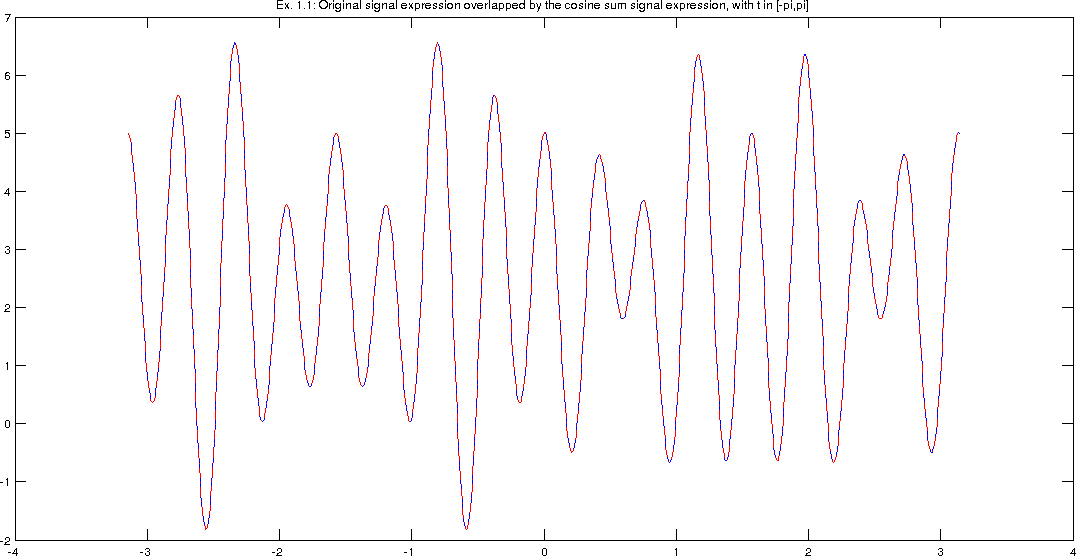
\includegraphics[scale=0.45]{images/ex11.png}
	\captionof{figure}{Original signal expression overlapped by the cosine sum signal expression, with $t \in [-\pi,\pi]$.}
	\label{fig:ex11}
\end{center}

\noindent Como é possível observar na figura \ref{fig:ex11}, a sobreposição das representações é perfeita.

\subsection{Exercise 1.2}
Fazendo uma simples substituição de $t$ por $n \, T_{s}$ na expressão obtida na alínea anterior obtém-se:
\begin{equation}
	x_{1}[n] = x_{1}(t) |_{t = n \, T_{s}} = \frac{5}{2} \, cos(0) + cos\left(9 \, n \, T_{s} + \frac{\pi}{2}\right) + cos\left(13 \, n \, T_{s} + \frac{3 \pi}{2}\right) + \frac{5}{2} \, cos(16 \, n \, T_{s})
\end{equation}

\subsection{Exercise 1.3}
O gráfico seguinte representa o sinal $x_1{1}(t)$ (a azul), para $t \in [-\pi, \pi]$ (com 500 elementos), sobreposto com o sinal $x_1{1}[n]$ (a vermelho) no mesmo intervalo, com um período de amostragem $T_ {s} = 0.1s$.

\begin{center}
	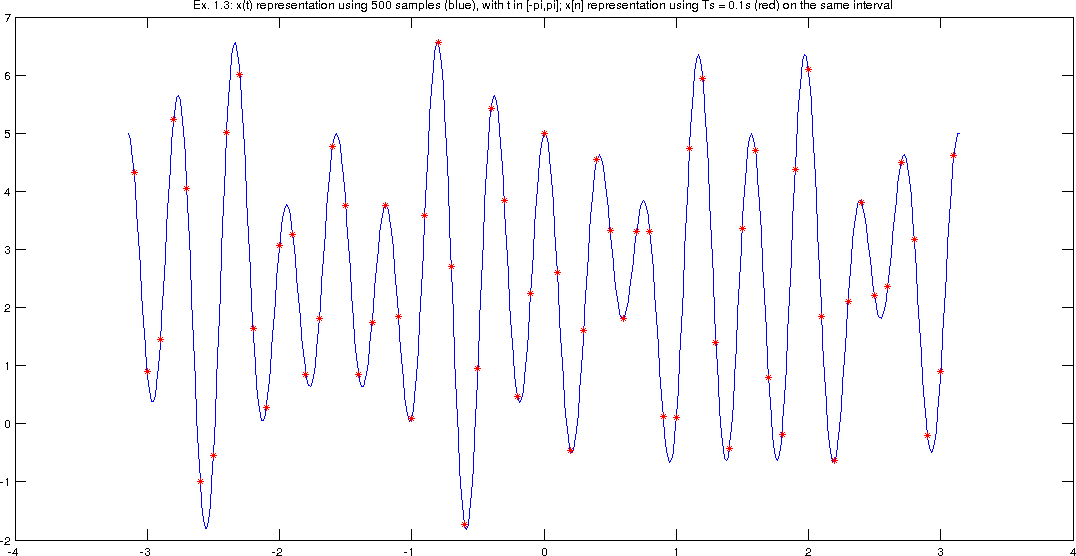
\includegraphics[scale=0.45]{images/ex13.png}
	\captionof{figure}{$x_1{1}(t)$ (blue), for $t \in [-\pi, \pi]$ (using 500 samples); $x_1{1}[n]$ (red) in the same interval, using $T_ {s} = 0.1s$.}
	\label{fig:ex13}
\end{center}

\noindent Como é possível observar na figura \ref{fig:ex13}, algumas amostras obtidas em $x_1{1}[n]$ apresentam um ligeiro desvio quando comparadas com o traçado do sinal $x_1{1}[n]$. Após alguma análise (incluíndo a soma das diferenças), concluímos que esse desvio se deve exclusivamente à perda de precisão decimal durante a criação do \emph{array} de espaçamento linear utilizado para o cálculo de $x_{1}(t)$.

% TODO

\section{Exercise 2}
\subsection{Exercise 2.1}
\indent \indent 

% ...


\section{Exercise 3}
\subsection{Exercise 3.1}
\indent \indent 

% ...


\section{Exercise 4}
\subsection{Exercise 4.1}
\indent \indent 

% ...


\section{Exercise 5}
\subsection{Exercise 5.1}
\indent \indent 

% ...


\section{Exercise 6}
\subsection{Exercise 6.1}
\indent \indent 

% ...

\end{document}
